\section{ The SABR model} \label{SABR_model}
In this chapter, we will first introduce the SABR model
 and explain how to determine the forward rate and 
 volatility using this model. We will then focus on 
 calculating implied volatility and pricing European 
 options with the SABR model. Finally, the chapter 
 will discuss methods for estimating the parameters 
 of the SABR model.
\\\\
The SABR (Stochastic Alpha, Beta, Rho) model marks a pivotal advancement 
in financial modeling, effectively addressing the significant limitations 
found in traditional methods like the Black Scholes model, which presupposes 
constant volatility. Developed in 2002 by Patrick Hagan, Deep Kumar, 
Andrew Lesniewski, and Diana Woodward, the SABR model is highly respected for 
its adeptness at managing the dynamic and unpredictable nature of market 
volatility.
\\\\
As a two-factor model, the SABR framework models both the forward rate 
(or asset price) and its volatility as a stochastic processes. This approach 
is vital as it incorporates a stochastic behavior in volatility, significantly 
improving the model's ability to capture the true, skewed, and heavy-tailed 
nature of financial market data. By allowing for volatility fluctuations, 
the SABR model provides a flexible and realistic framework for pricing 
derivatives, proving especially useful for options with long maturities where 
the assumption of constant volatility falls short \cite{Smile}.
\subsection{Specification for the SABR model}
The main different between the SABR model and the 
Black Scholes model is the assumptions regrading the 
volatility, as mentioned earlier. In the Black Scholes 
model the volatility is a assumed to be constant and 
in the SABR model the volatility evolve as a function
of time, t, the strike price, K, and the current
forward price, $f_t$. Futhermore the volatility itself
is random. So we chose the unknown coefficient $C(t,*)$
to be $\hat{\alpha} \hat{F}^{\beta}$, where the 
"volatility" $\hat{\alpha}$ is a stochastic process itself. 
The extra randomness is scaled thought the inclusion 
of a "volatility of volatility" parameter $\nu$.
\\\\
Now we will formulate the SABR model mathematically. 
The SABR model consist of a dynamic for the forward price
and one for the volatility, since the SABR model is a 
two-factor model. The SABR model also formulate the 
how the two process is correlated. 
\begin{align}
    df_t &= \alpha_t f_t^\beta dW_t^1, \quad \quad \hat{F}(0)=f   \label{f_dyn}\\
    d\alpha_t &= \nu \alpha_t dW_t^2, \quad \quad \hat{\alpha}(0)=\alpha \label{sigma_dyn}
\end{align}
where $W_t^{1}$ and $W_t^{2}$ are two correlated Wiener 
process and it is assmued that \cite{Smile}.
\begin{align}
    dW_t^{1}dW_t^{2}=\rho dt
\end{align}
So we have that 
parameters in the SABR model is as follows, $\alpha$ represents the initial volatility level
, $\nu$ represents the volatility of volatility, or the rate at which volatility itself changes
, $\beta$ represents the elasticity of the volatility; a common practice is to fix beta based on the underlying asset 
and as mentioned $\rho$ is the correlations between the 
two Wiener process, the asset price and its volatility. 
\\\\
So the SABR model is characterized by the stochastic process $\alpha_t$,
the parameter $\beta$, and the correlation coefficient $\rho$,
which is also reflected in its name - Stochastic Alpha Bete Rho.
In a specific variant of the SABR model, 
by setting $\beta = 1 $ and $\nu = 0$, the model reverts 
to the classic Black Scholes framework. 
This configuration leads to a constant volatility, 
denoted $\alpha_0 $, 
and a forward process where returns follow a 
normal distribution with a mean of zero and a standard 
deviation of $\alpha_0 \sqrt{t}$. So now the SABR model
has been introduced and the analysis will continuing forward 
to how to price a swaption using the SABR model to determine the implied
volatility.
\subsection{Simulation the SABR model}
In this section a short view on how the process for the forward price and the volatility develops over times will be covered. 
To provide the intuition on how the dynamic listed in \autoref{f_dyn} and \autoref{sigma_dyn} behave, the dynamics is simulated ten times
for some chosen parameters is listed in \autoref{tab:parameters_sim_sabr}. 
The simulated paths is illustrated in \autoref{fig:sim_f_and_sigma} below. 
From \autoref{fig:sim_f_and_sigma} we see that the dynamics are driven by the randomness in the Wiener process and 
it develops from the initial value of the forward price and volatility.
\begin{table}[H]
    \centering
    \begin{tabular}{ccc}
      \toprule
      \textbf{Parameter} & \textbf{Parameter explanation} & \textbf{Value} \\
      \midrule
      $F_0$ & Initial forward rate or asset price & 100 \\
      $\alpha_0$ & Initial volatility  & 0.2 \\
      $\beta$ & Elasticity parameter & 0.5 \\
      $\nu$ & Volatility of the volatility parameter & 0.25 \\
      $\rho$ & Correlation between the asset price and its volatility & -0.4 \\
      \bottomrule
    \end{tabular}
    \caption{Summary of Parameters used for simulating the SABR model}
    \label{tab:parameters_sim_sbar}
\end{table}
\noindent

\begin{figure}[H]
    \centering
    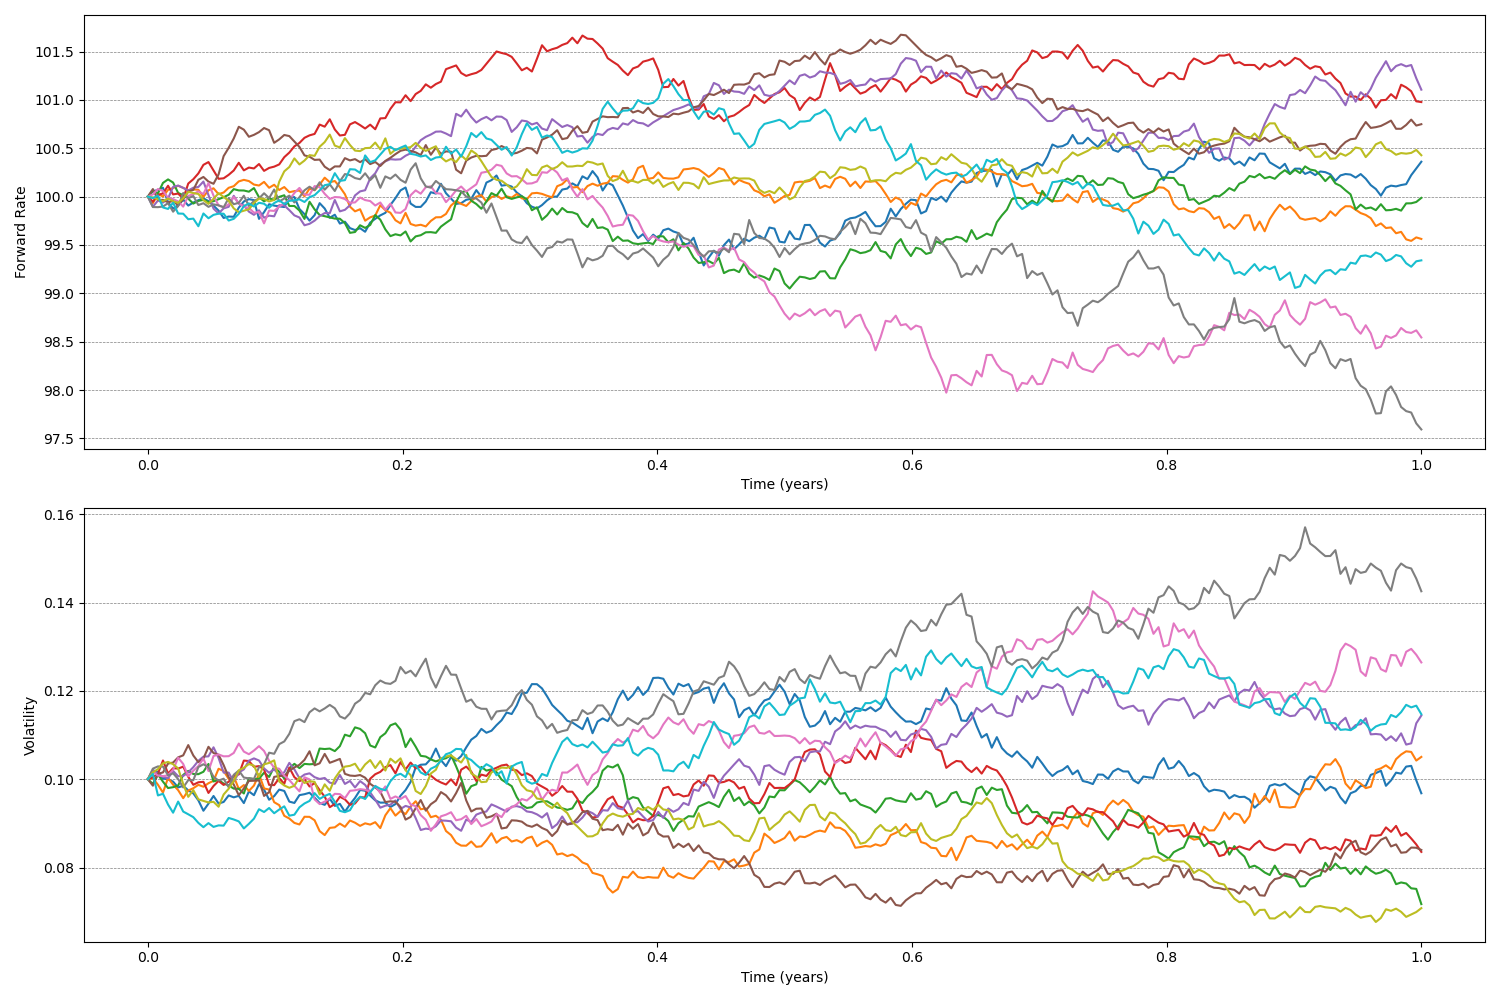
\includegraphics[width=0.8\textwidth]{/Users/nannaingemannohrt/Desktop/master_thesis/main/plots/sim_f_and_sigma.png}
    \caption{Ten simulated paths for the forward rate and the volatility in the SABR model.}
    \label{fig:sim_f_and_sigma}
\end{figure}
\noindent
\subsection{SABR Implied Volatility and Option Prices}
Before we are able to move forward with the analysis,
we need to formulate how to determine implied volatility in the SABR model. 
But these calculations are out of the scope for this analysis,
so we will used the formula in the paper Managing Smile Risk 
of Hagen (2002) \cite{Smile}. The paper states that
under the SABR model, the prices of European options 
is given by Black formula in \autoref{sabr1} to \autoref{sabr3}
below
\begin{align}
    V_{\text{call}} &= D(t_{\text{set}})fN(d_1) - KN(d_2),  \label{sabr1}\\
    V_{\text{put}} &= V_{\text{call}} + D(t_{\text{set}})[K - f], \label{sabr2}
\end{align}
with
\begin{equation}
    d_{1,2} = \frac{\log \frac{f}{K} \pm \frac{1}{2}\sigma_B^2 t_{\text{ex}}}{\sigma_B \sqrt{t_{\text{ex}}}}, \label{sabr3}
\end{equation}
where the implied volatility $\sigma_B(f, K)$ is given by
\begin{equation}
    \sigma_B(K, f) = \frac{\alpha}{(fK)^{(1-\beta)/2}} \left\{ 1 + \frac{(1-\beta)^2}{24} \log^2 \frac{f}{K} + \frac{(1-\beta)^4}{1920} \log^4 \frac{f}{K} + \ldots \right\} \left( \frac{z}{x(z)} \right).
    \label{sigma_B}
\end{equation}
where
\begin{align}
    z &= \frac{\nu}{\alpha}(fK)^{(1-\beta)/2} \log \frac{f}{K}, \\
\end{align}
and x(z) is defined by
\begin{align}
    x(z) &= \log \left\{ \frac{\sqrt{1-2\rho z + z^2} + z - \rho}{1 - \rho} \right\}.
\end{align}
For the special case of at-the-money (ATM) options, options strike at $K = f$, this formula reduces to
\begin{equation}
    \sigma_{ATM} = \sigma_B(f, f) = \frac{\alpha}{f^{1-\beta}} \left\{ 1 + \left( \frac{(1-\beta)^2}{24} \frac{\alpha^2}{f^{2-2\beta}} + \frac{\rho \beta \nu}{4} \frac{\alpha}{f^{1-\beta}} + \frac{2-3\rho^2}{24} \nu^2 \right) t_{\text{ex}} + \ldots \right\}.
    \label{sigma_ff}
\end{equation}
\\
So we have that the parameters $\alpha, \beta, \nu$ and $\rho$  in the SABR model is estimated and the implied volatility $\sigma_B$
is a function of the forward price and the strike. Now that we have a simplified formula for the implied 
volatility from the SABR model, we can start analyzing 
how the model works. We will do this by continuing your
analysis with investigating how the different parameters 
affects implied volatility in the SABR model. 

\subsection{Investigating the parameters of the SABR model}
In this section, we will explore the parameters of the SABR model. This analysis will offer insights into 
how different parameters influence the behavior of implied volatility. We will conduct this investigation using 
the closed-form solution established in the previous section. Our study will be build on  \autoref{sigma_B} and 
\autoref{sigma_ff}, where we will test various parameter values. To see how changes in the different parameters
affects on the implied volatility smile so realistic as possible we fix the values of the parameters.
Below in \autoref{tab:parameters} the chosen value of the parameters are listed, together with a short
explain of the parameters. Then the study is performed by changing the parameters one by one, to illustrate the 
isolated effect of the parameters. 

\begin{table}[H]
    \centering
    \begin{tabular}{ccc}
      \toprule
      \textbf{Parameter} & \textbf{Parameter explanation} & \textbf{Value} \\
      \midrule
      $f$ & Initial forward rate or asset price & 100 \\
      $T$ & Time to maturity & 1 \\
      $K$ & Strike & $K \in (80,120)$ \\
      $\alpha_0$ & Initial level of volatility & 0.1 \\
      $\beta$ & Elasticity of the volatility & 0.5 \\
      $\rho$ & Correlation between the asset price and its volatility & -0.4 \\
      $\nu$ & Volatility of the volatility parameter & 0.25 \\
      \bottomrule
    \end{tabular}
    \caption{Summary of Parameters}
    \label{tab:parameters}
\end{table}
\noindent
We will start the study with investigating how $\alpha_0$ affects the volatility smile in the SABR model. 
First we note that the fix value of $\alpha_0$ is $0.1$ Hereafter we adjust the value of $\alpha_0$ to $0.05$ and $0.15$,
where the other parameters are kept fixed as listed in \autoref{tab:parameters} above. So have change the parameter
up and down from the initial value of $\alpha_0$.
We note that the parameter $\alpha_0$
represents "the initial level of volatility" as it is the starting point for the stochastic volatility process. 
Below in \autoref{fig:alpha} the volatility smile is illustrated for three different value of $\alpha_0$. 
From \autoref{fig:alpha} we see that the up and down movements don't change the shape of the volatility smile, 
it only shifts the volatility smile respectively up and down given the movement in $\alpha_0$.
\begin{figure}[H]
    \centering
    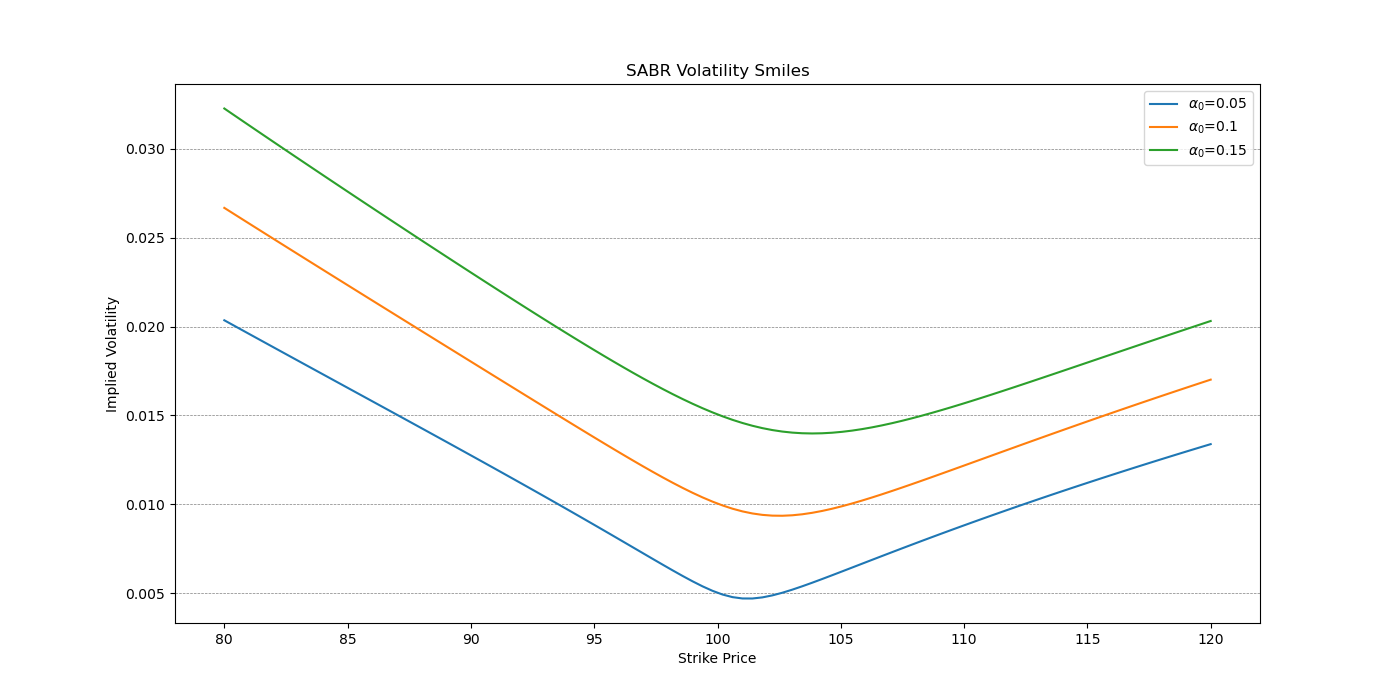
\includegraphics[width=0.7\textwidth]{/Users/nannaingemannohrt/Desktop/master_thesis/main/plots/SABR1_alpha.png}
    \caption{SABR model volatility smiles at various $\alpha_0$ levels}
    \label{fig:alpha}
\end{figure}
\noindent
Then we will continue the study of the parameters affects by looking into shift in the beta value in the SABR model.
Aging we shift the value of $\beta$ up and down from the fixed beta in \autoref{tab:parameters}. So we will look at $\beta$ equal to $0.3$,
$0.5$ (the fix beta) and $0.7$. 
Although not explicitly constrained in the original article by Hagan et al. (2002), we restrict $\beta$ to the range $[0, 1]$. 
Choosing a $\beta$ less than 0 would lead to an illogical scenario where higher forward prices F result in a smaller 
relative change in the process $f_t$, thus we set the lower limit at $\beta \leq 0$. Similarly, a $\beta$ greater than 1 would 
suggest that the expected deviation from the current state of $F_t$ exceeds the product of volatility and the current 
forward level (times $\alpha_0 \sqrt{t}$), which is also impractical. Therefore, we set the upper limit at $\beta \geq 0$.
\\\\
Below in \autoref{fig:beta} the volatility smile in the SABR model for the different beta values are illustrated.
From \autoref{fig:beta} we see a small effect of the curvature of the volatility smile. We also not that for higher 
beta the shift is larger, than for lower beta. We also note that the change in the beta parameter is more present in 
the left side from of strike value at-the-money (ATM). Other than that we wee the same patterns from the change in 
the alpha parameter, namely the up and down shifts in the volatility smile, respectively to the movement in the 
beta parameter.
\begin{figure}[H]
    \centering
    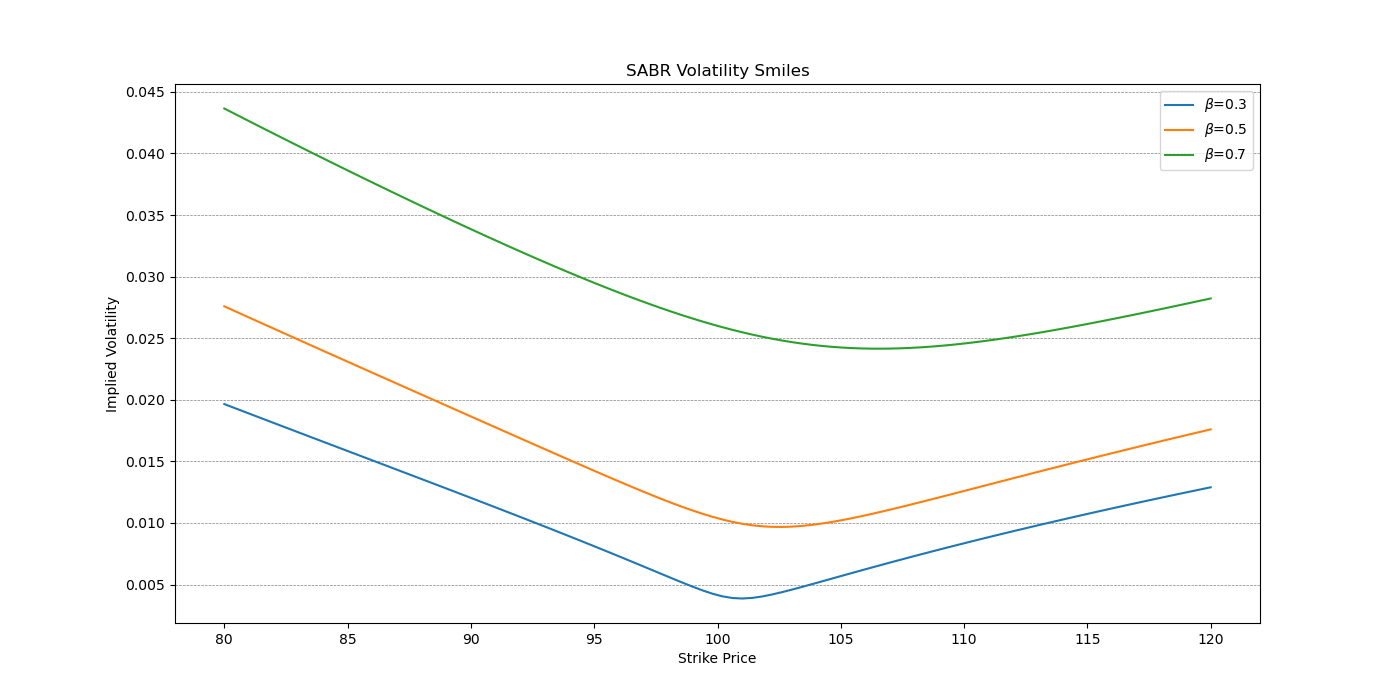
\includegraphics[width=0.7\textwidth]{/Users/nannaingemannohrt/Desktop/master_thesis/main/plots/SABR_beta.png}
    \caption{SABR model volatility smiles at various $\beta$ levels}
    \label{fig:beta}
\end{figure}
\noindent
Moving forward we will shift the $\nu$ parameter, which can be describe as the volatility of the volatility parameter.
Again we shift the $\nu$ parameter up and down from the fixed $\nu$ parameter listed in \autoref{tab:parameters}.
The volatility smile calculated from the SABR for the different $\nu$ parameters are illustrated in \autoref{fig:nu} below.
A very clear pattern emerges, namely that the parameter $\nu$ controls the curvature of the volatility smile in
the SABR model. When we look at the shifts in the beta parameter we make a comment that it made small changes in 
the curvature. But after this part of the analysis, we clearly see that the curvature is determine from the value
of $\nu$. Which makes good sense, when we think of the interpretation of the parameter describe before.
We also note that when $\nu$  increasing the level of the implied volatility for the 
out-of-the-money (OTM) strikes also increase and vise vera.
\\\\
Then we look at the parameter for the correlation between the asset price and its volatility, namely $\rho$.
So we have that $\rho$ is the correlation between to two Wiener process in the SABR model, hence we have
that $\rho$ is bounded and takes values between $-1$ and $1$. In \autoref{fig:rho} the shifted valus of $\rho$
from the fixed value is illustrated. 
We see that higher positive correlations generally show a decreasing trend in implied volatility with an increase in strike price, 
while strong negative correlations can cause the implied volatility to increase with strikes there are in-the-money (ITM).
We alo note that when the correlation is close to zero the smile is more symmetric around the ATM strike. 
So in total we see that the correlation parameter $\rho$ has a significantly affects on the shape and slope of
the volatility smile in the SABR model, and hence on the implied volatilities values.
\begin{figure}[H]
    \centering
    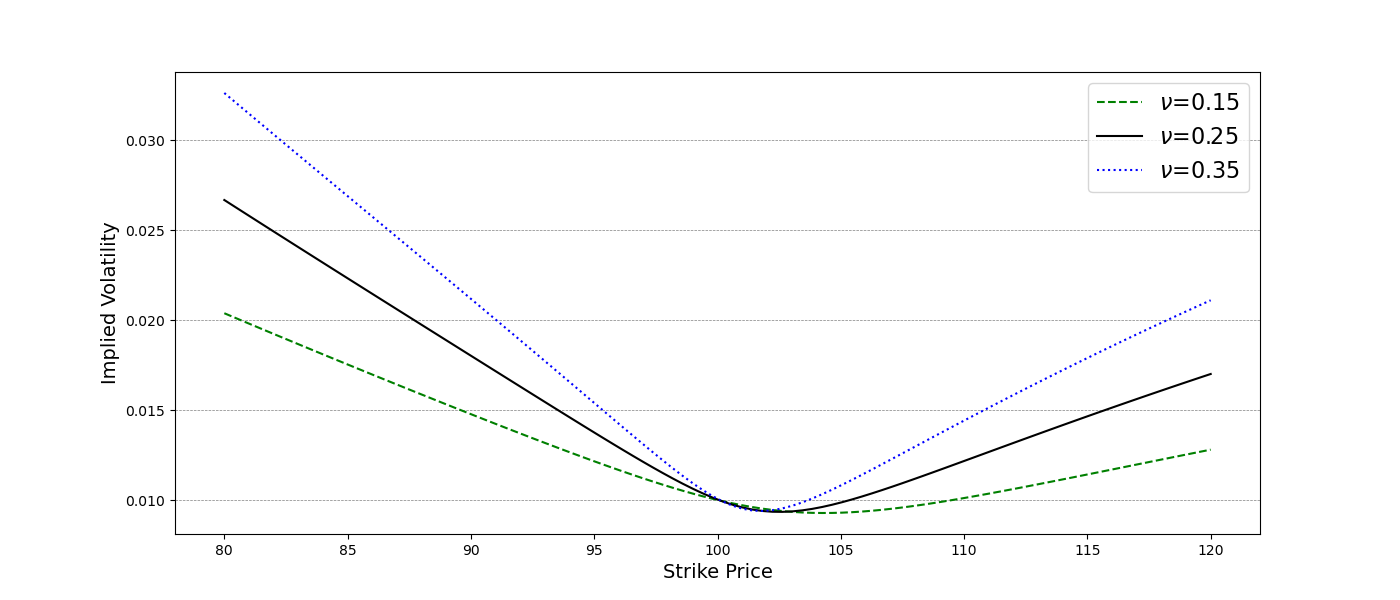
\includegraphics[width=0.7\textwidth]{/Users/nannaingemannohrt/Desktop/master_thesis/main/plots/SABR_nu.png}
    \caption{SABR model volatility smiles at various $\nu$ levels}
    \label{fig:nu}
\end{figure}

\begin{figure}[H]
    \centering
    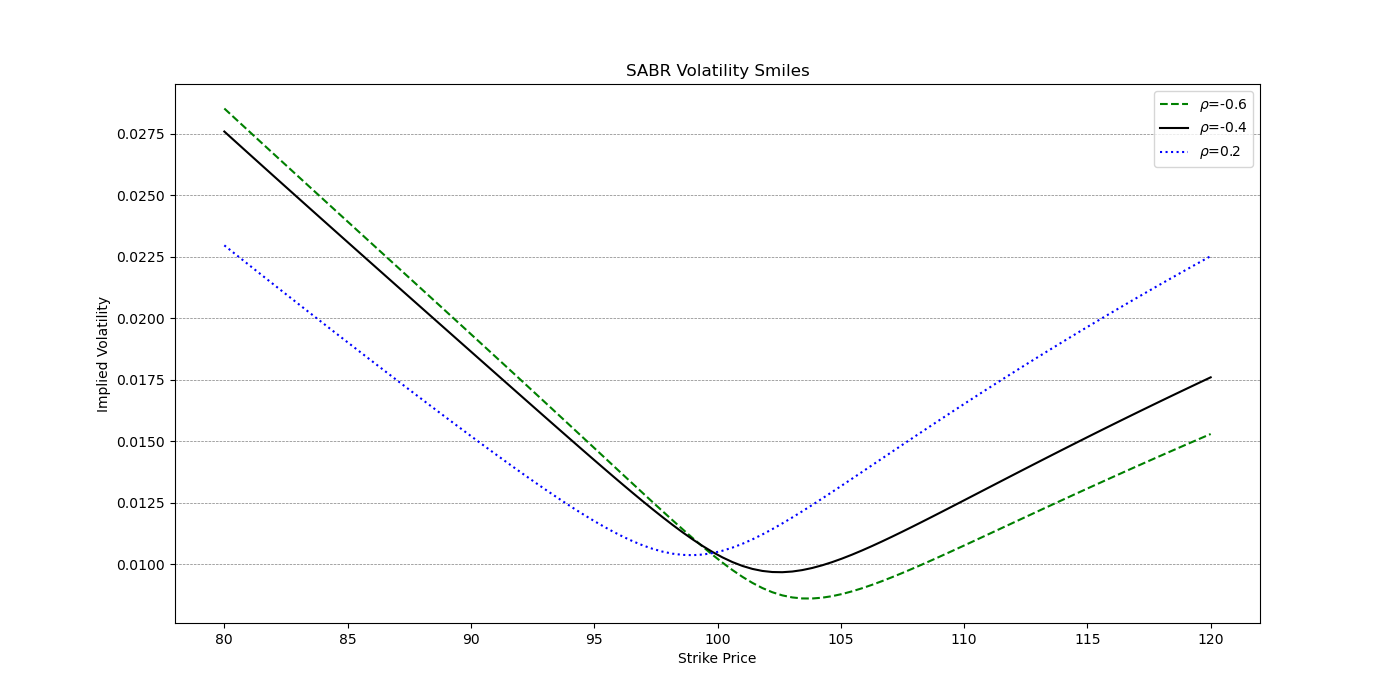
\includegraphics[width=0.7\textwidth]{/Users/nannaingemannohrt/Desktop/master_thesis/main/plots/SABR_rho.png}
    \caption{SABR model volatility smiles at various $\rho$ levels}
    \label{fig:rho}
\end{figure}

\begin{figure}[H]
    \centering
    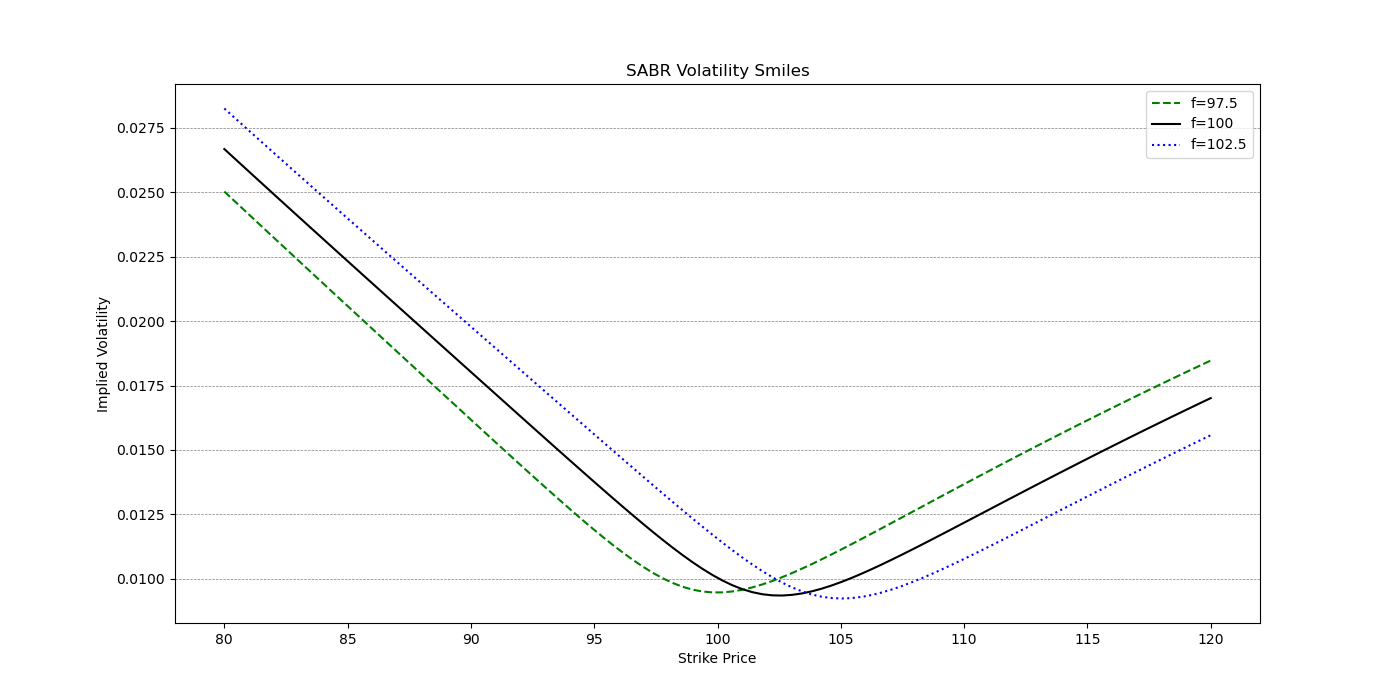
\includegraphics[width=0.7\textwidth]{/Users/nannaingemannohrt/Desktop/master_thesis/main/plots/SABR_f.png}
    \caption{SABR model volatility smiles at various f levels}
    \label{fig:f}
\end{figure}
\noindent
\\\\
Finally we will investigate how the forward price, f, affect the volatility smile in the SABR model. 
The same procedure as for the other parameters will be used. So in \autoref{fig:f} the volatility smile
for the forward prices are illustrated. We see that the slope, shape and curvature is retained, when there
is only change in the forward price. Which is as we expected given how the forward price, f, enters in the closed
solution for the implied volatility in \autoref{sigma_B} and \autoref{sigma_ff}.
\\\\
To summarize this section provides knowledge of the impact of the various parameters in the closed-form solution
for the implied volatility in the SABR model. This knowledge gives a good idea of how that model works, and 
positions us better to understand estimation of the model. So now we have look the closed-form solution and 
now the next step of our analysis is to move forward to estimating the parameters in the SABR model.
\newpage
\subsection{Estimating Parameters in the SABR model}
\subsection{Fitting a volatility smile using the SABR model}
